\documentclass[11pt,oneside,a4paper]{scrartcl}

\usepackage[left=2cm,right=2cm,top=1.5cm,bottom=1.5cm,includeheadfoot,]{geometry}
\usepackage{enumitem}
\usepackage{graphicx}
\usepackage{fancyhdr}
\usepackage{hyperref}
\usepackage{listings}
\usepackage{gensymb}


\pagestyle{fancy}
\fancyhf{}

\fancyhead[L]{Foundationcourse 2016}
\fancyhead[R]{12.09.2016}

\renewcommand{\headrulewidth}{0.5pt}

\fancyfoot[L]{Markus Wiktorin, Aniruddha Pal}
\fancyfoot[R]{\thepage}

\renewcommand{\footrulewidth}{0.5pt}

\begin{document}
\section*{Lego Project Description}

\subsection*{Task: Line following}
The robot has to follow a black line with complex turns. Robots will be timed on 
different tracks. If an intersection occurs, the robot has to go straight.

\subsection*{Our strategy}
We build a robot with two motors with attached wheels. A third flexible wheel at the rear makes it possible to turn the robot by assigning different speeds to the motors. In the front we will attach a light sensor which is capable of deciding whether the ground is black or white. We use the sensor in order to follow the black line.\\
We start by going straight until we find the black line. The the robot will will move forward as long as the underground stays black. If it is not black any more, the robot lost the line and should turn left or right in order to find it again. It will start turning left until it finds a line or it turned more than 120$^{\circ}$ because we don't want it to turn to go back to the line. If it couldn't find the line it will turn right, again at most 120$^{\circ}$. The robot should remember whether it found the line left or right and the next time it looses the line it will start looking for it in the same direction. This way, long turns will be followed faster.

\subsection*{Algorithm}
In the following we will describe our algorithm with pseudocode:
\begin{lstlisting}
lastDirection := left
while (underground is white) {
	move forward
}
// At this point the robot is on the line
while (true) {
	while (underground is black) {
		move forward
	}
	// At this point the robot lost the line
	while (underground is white AND turnAngle < 120) {
		turn lastDirection
	}
	if (underground is white) {
		turn back
		while (underground is white AND turnAngle < 120) {
			turn !lastDirection
		}
		lastDirection := !lastDirection
	}
	if (underground is white) {
		error lost line
	}
}
\end{lstlisting}

\begin{center}
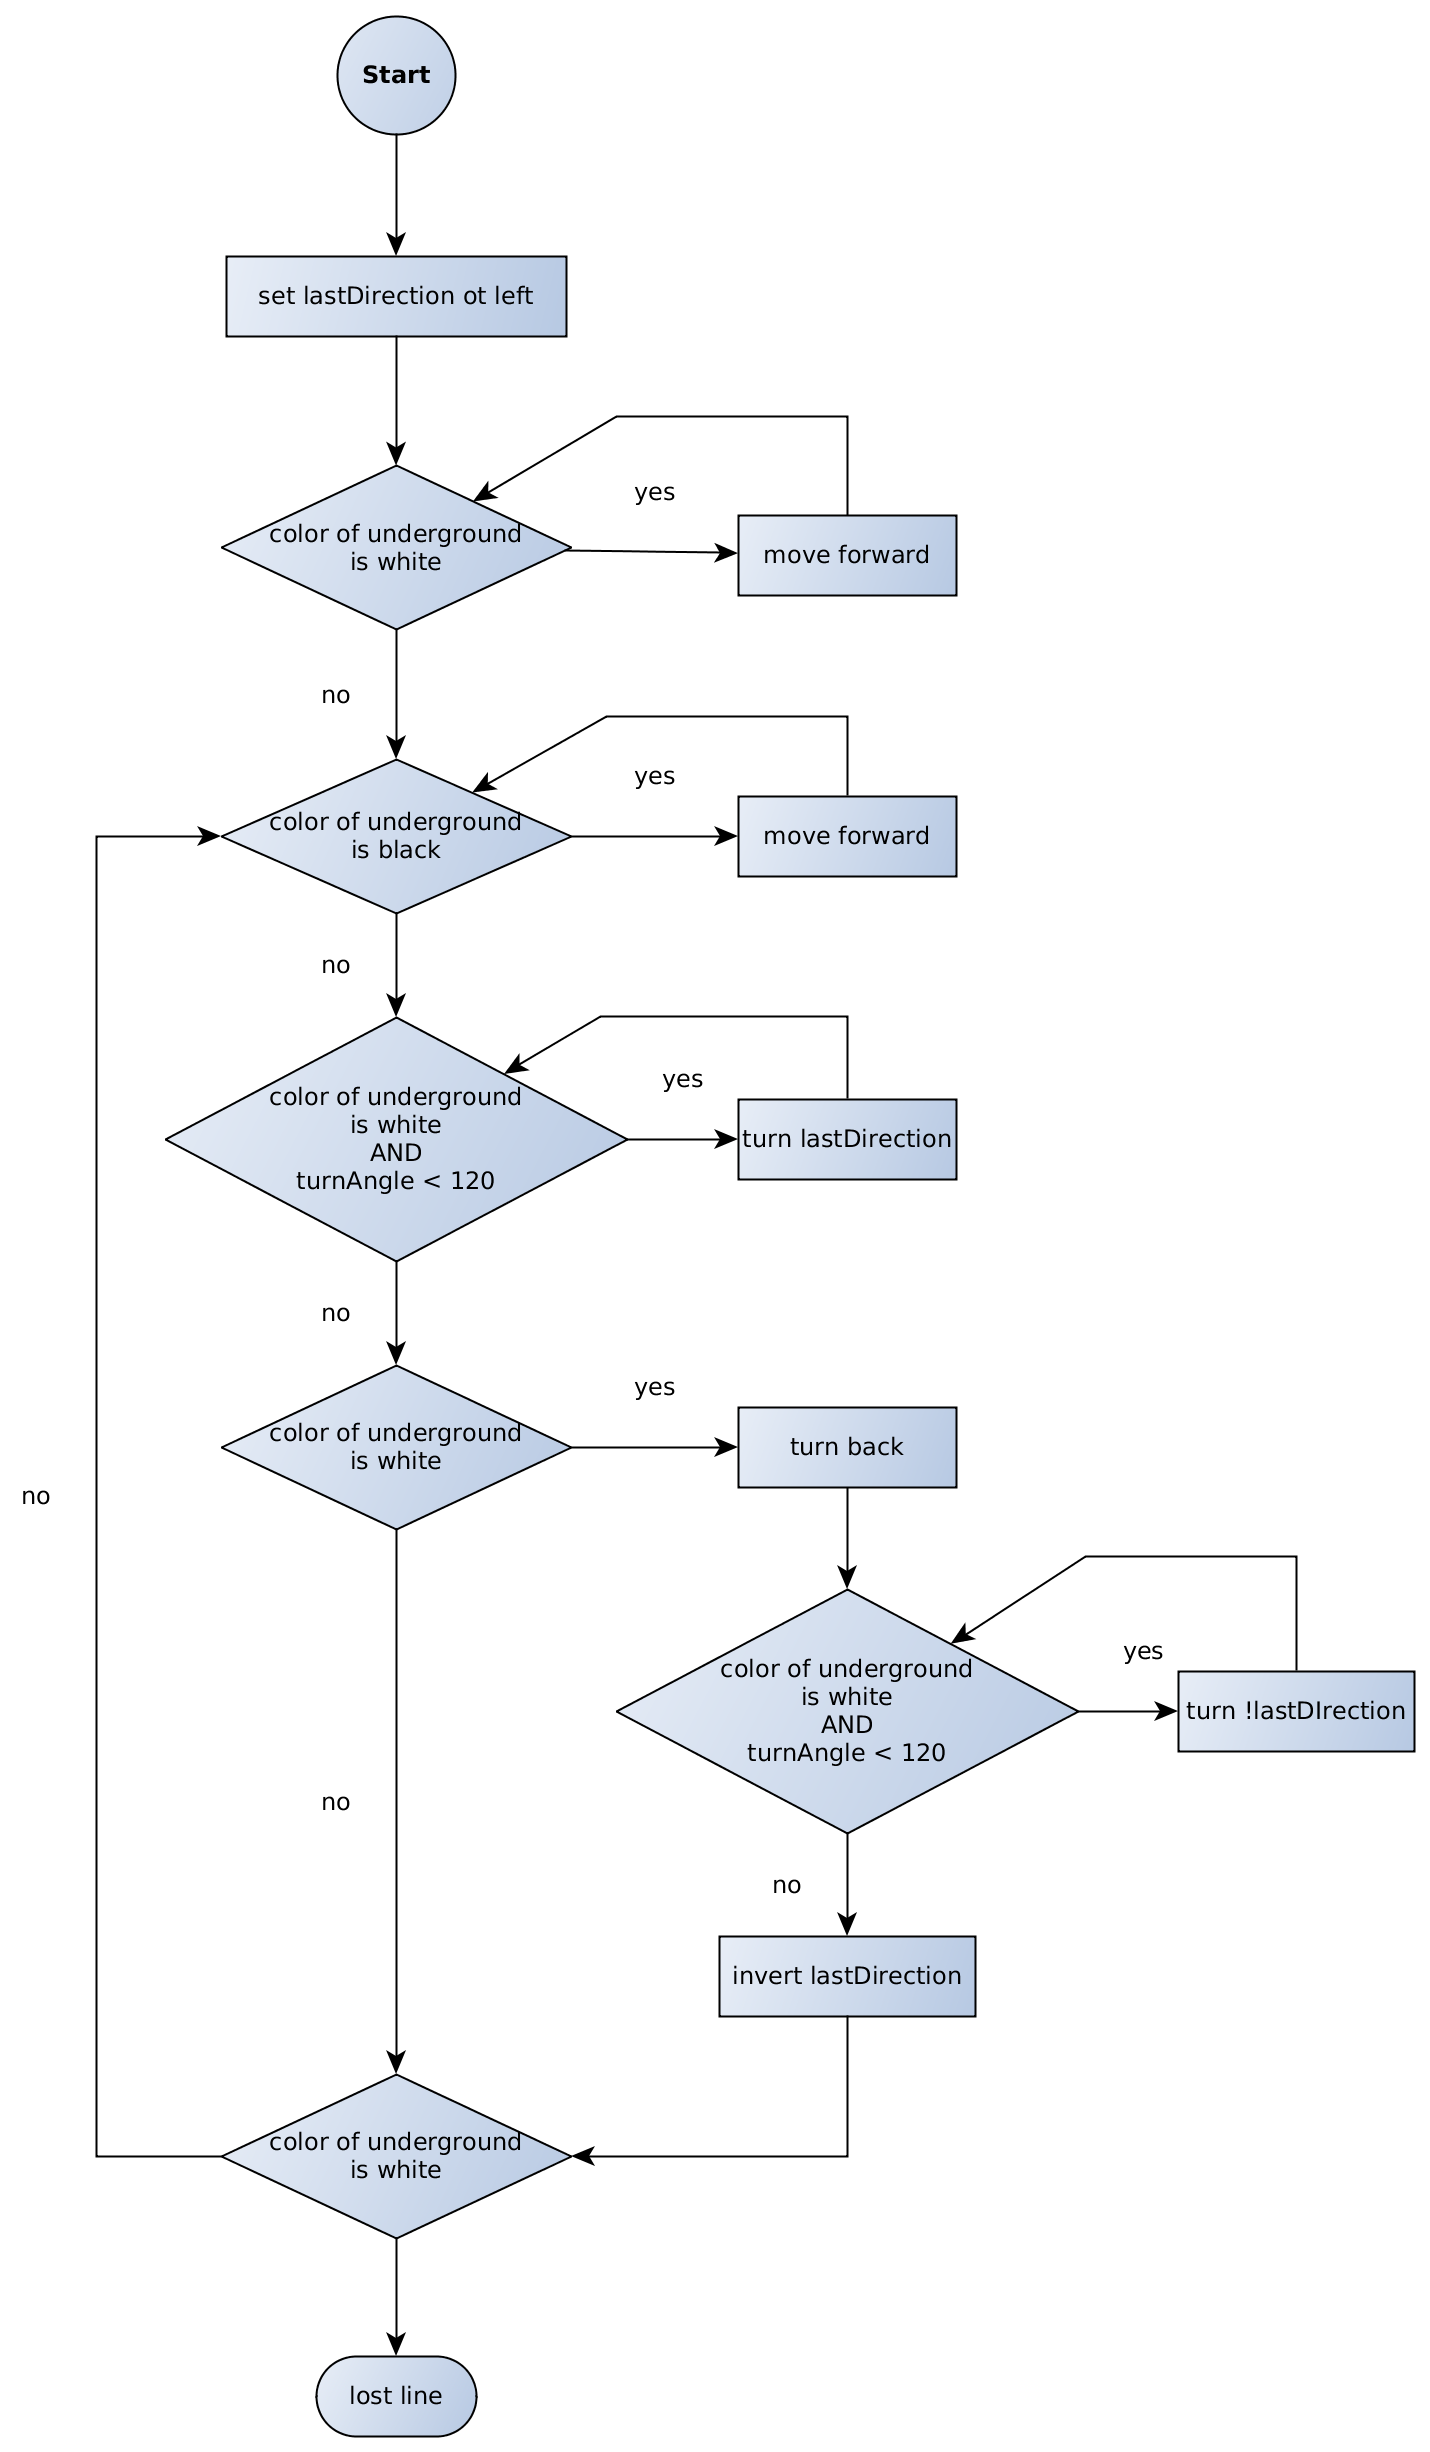
\includegraphics[width=\textwidth,height=\textheight,keepaspectratio]{flowChart.png}
\end{center}

\end{document}